\documentclass[twoside]{book}

% Packages required by doxygen
\usepackage{fixltx2e}
\usepackage{calc}
\usepackage{doxygen}
\usepackage[export]{adjustbox} % also loads graphicx
\usepackage{graphicx}
\usepackage[utf8]{inputenc}
\usepackage{makeidx}
\usepackage{multicol}
\usepackage{multirow}
\PassOptionsToPackage{warn}{textcomp}
\usepackage{textcomp}
\usepackage[nointegrals]{wasysym}
\usepackage[table]{xcolor}

% Font selection
\usepackage[T1]{fontenc}
\usepackage[scaled=.90]{helvet}
\usepackage{courier}
\usepackage{amssymb}
\usepackage{sectsty}
\renewcommand{\familydefault}{\sfdefault}
\allsectionsfont{%
  \fontseries{bc}\selectfont%
  \color{darkgray}%
}
\renewcommand{\DoxyLabelFont}{%
  \fontseries{bc}\selectfont%
  \color{darkgray}%
}
\newcommand{\+}{\discretionary{\mbox{\scriptsize$\hookleftarrow$}}{}{}}

% Page & text layout
\usepackage{geometry}
\geometry{%
  a4paper,%
  top=2.5cm,%
  bottom=2.5cm,%
  left=2.5cm,%
  right=2.5cm%
}
\tolerance=750
\hfuzz=15pt
\hbadness=750
\setlength{\emergencystretch}{15pt}
\setlength{\parindent}{0cm}
\setlength{\parskip}{3ex plus 2ex minus 2ex}
\makeatletter
\renewcommand{\paragraph}{%
  \@startsection{paragraph}{4}{0ex}{-1.0ex}{1.0ex}{%
    \normalfont\normalsize\bfseries\SS@parafont%
  }%
}
\renewcommand{\subparagraph}{%
  \@startsection{subparagraph}{5}{0ex}{-1.0ex}{1.0ex}{%
    \normalfont\normalsize\bfseries\SS@subparafont%
  }%
}
\makeatother

% Headers & footers
\usepackage{fancyhdr}
\pagestyle{fancyplain}
\fancyhead[LE]{\fancyplain{}{\bfseries\thepage}}
\fancyhead[CE]{\fancyplain{}{}}
\fancyhead[RE]{\fancyplain{}{\bfseries\leftmark}}
\fancyhead[LO]{\fancyplain{}{\bfseries\rightmark}}
\fancyhead[CO]{\fancyplain{}{}}
\fancyhead[RO]{\fancyplain{}{\bfseries\thepage}}
\fancyfoot[LE]{\fancyplain{}{}}
\fancyfoot[CE]{\fancyplain{}{}}
\fancyfoot[RE]{\fancyplain{}{\bfseries\scriptsize Generated by Doxygen }}
\fancyfoot[LO]{\fancyplain{}{\bfseries\scriptsize Generated by Doxygen }}
\fancyfoot[CO]{\fancyplain{}{}}
\fancyfoot[RO]{\fancyplain{}{}}
\renewcommand{\footrulewidth}{0.4pt}
\renewcommand{\chaptermark}[1]{%
  \markboth{#1}{}%
}
\renewcommand{\sectionmark}[1]{%
  \markright{\thesection\ #1}%
}

% Indices & bibliography
\usepackage{natbib}
\usepackage[titles]{tocloft}
\setcounter{tocdepth}{3}
\setcounter{secnumdepth}{5}
\makeindex

% Hyperlinks (required, but should be loaded last)
\usepackage{ifpdf}
\ifpdf
  \usepackage[pdftex,pagebackref=true]{hyperref}
\else
  \usepackage[ps2pdf,pagebackref=true]{hyperref}
\fi
\hypersetup{%
  colorlinks=true,%
  linkcolor=blue,%
  citecolor=blue,%
  unicode%
}

% Custom commands
\newcommand{\clearemptydoublepage}{%
  \newpage{\pagestyle{empty}\cleardoublepage}%
}

\usepackage{caption}
\captionsetup{labelsep=space,justification=centering,font={bf},singlelinecheck=off,skip=4pt,position=top}

%===== C O N T E N T S =====

\begin{document}

% Titlepage & ToC
\hypersetup{pageanchor=false,
             bookmarksnumbered=true,
             pdfencoding=unicode
            }
\pagenumbering{roman}
\begin{titlepage}
\vspace*{7cm}
\begin{center}%
{\Large My Project }\\
\vspace*{1cm}
{\large Generated by Doxygen 1.8.11}\\
\end{center}
\end{titlepage}
\clearemptydoublepage
\tableofcontents
\clearemptydoublepage
\pagenumbering{arabic}
\hypersetup{pageanchor=true}

%--- Begin generated contents ---
\chapter{File Index}
\section{File List}
Here is a list of all files with brief descriptions\+:\begin{DoxyCompactList}
\item\contentsline{section}{\hyperlink{Lab1_8c}{Lab1.\+c} }{\pageref{Lab1_8c}}{}
\end{DoxyCompactList}

\chapter{File Documentation}
\hypertarget{Bubble_8c}{}\section{Bubble.\+c File Reference}
\label{Bubble_8c}\index{Bubble.\+c@{Bubble.\+c}}
{\ttfamily \#include $<$stdio.\+h$>$}\\*
Include dependency graph for Bubble.\+c\+:
\nopagebreak
\begin{figure}[H]
\begin{center}
\leavevmode
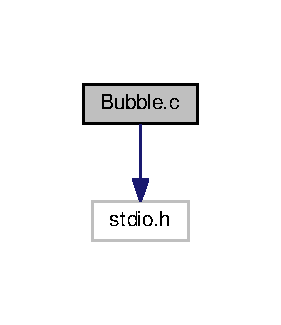
\includegraphics[width=135pt]{Bubble_8c__incl}
\end{center}
\end{figure}
\subsection*{Macros}
\begin{DoxyCompactItemize}
\item 
\#define \hyperlink{Bubble_8c_a5de5d183f9a6a8d53316f743e1ca6dc2}{N\+M\+AX}~10
\end{DoxyCompactItemize}
\subsection*{Functions}
\begin{DoxyCompactItemize}
\item 
int \hyperlink{Bubble_8c_a3ecb30d4a656177910184bb2489afe90}{get\+Int\+Array} (int a\mbox{[}$\,$\mbox{]}, int nmax, int sentinel)
\item 
void \hyperlink{Bubble_8c_a84fa1f32b691605131bea795bba242bd}{print\+Int\+Array} (int a\mbox{[}$\,$\mbox{]}, int n)
\item 
void \hyperlink{Bubble_8c_aa3d39f5a62aa262672371153433dec0b}{bubble\+Sort} (int a\mbox{[}$\,$\mbox{]}, int n)
\item 
int \hyperlink{Bubble_8c_a840291bc02cba5474a4cb46a9b9566fe}{main} (void)
\end{DoxyCompactItemize}


\subsection{Macro Definition Documentation}
\index{Bubble.\+c@{Bubble.\+c}!N\+M\+AX@{N\+M\+AX}}
\index{N\+M\+AX@{N\+M\+AX}!Bubble.\+c@{Bubble.\+c}}
\subsubsection[{\texorpdfstring{N\+M\+AX}{NMAX}}]{\setlength{\rightskip}{0pt plus 5cm}\#define N\+M\+AX~10}\hypertarget{Bubble_8c_a5de5d183f9a6a8d53316f743e1ca6dc2}{}\label{Bubble_8c_a5de5d183f9a6a8d53316f743e1ca6dc2}


\subsection{Function Documentation}
\index{Bubble.\+c@{Bubble.\+c}!bubble\+Sort@{bubble\+Sort}}
\index{bubble\+Sort@{bubble\+Sort}!Bubble.\+c@{Bubble.\+c}}
\subsubsection[{\texorpdfstring{bubble\+Sort(int a[], int n)}{bubbleSort(int a[], int n)}}]{\setlength{\rightskip}{0pt plus 5cm}void bubble\+Sort (
\begin{DoxyParamCaption}
\item[{int}]{a\mbox{[}$\,$\mbox{]}, }
\item[{int}]{n}
\end{DoxyParamCaption}
)}\hypertarget{Bubble_8c_aa3d39f5a62aa262672371153433dec0b}{}\label{Bubble_8c_aa3d39f5a62aa262672371153433dec0b}

\begin{DoxyCode}
69 \{
70   \textcolor{keywordtype}{int} lcv;
71   \textcolor{keywordtype}{int} limit = n-1;
72   \textcolor{keywordtype}{int} temp;
73   \textcolor{keywordtype}{int} lastChange;
74   
75   \textcolor{keywordflow}{while} (limit) \{
76     lastChange = 0;
77     \textcolor{keywordflow}{for} (lcv=0;lcv<limit;lcv++)
78       \textcolor{comment}{/* Notice that the values in positions LIMIT+1 .. N are in
}
79 \textcolor{comment}{       * their final position, i.e. they are sorted right */}
80     \textcolor{keywordflow}{if} (a[lcv]>a[lcv+1]) \{
81       temp = a[lcv];
82       a[lcv] = a[lcv+1];
83       a[lcv+1] = temp;
84       lastChange = lcv;
85     \}
86     limit = lastChange;
87   \}
88 \}\end{DoxyCode}
\index{Bubble.\+c@{Bubble.\+c}!get\+Int\+Array@{get\+Int\+Array}}
\index{get\+Int\+Array@{get\+Int\+Array}!Bubble.\+c@{Bubble.\+c}}
\subsubsection[{\texorpdfstring{get\+Int\+Array(int a[], int nmax, int sentinel)}{getIntArray(int a[], int nmax, int sentinel)}}]{\setlength{\rightskip}{0pt plus 5cm}int get\+Int\+Array (
\begin{DoxyParamCaption}
\item[{int}]{a\mbox{[}$\,$\mbox{]}, }
\item[{int}]{nmax, }
\item[{int}]{sentinel}
\end{DoxyParamCaption}
)}\hypertarget{Bubble_8c_a3ecb30d4a656177910184bb2489afe90}{}\label{Bubble_8c_a3ecb30d4a656177910184bb2489afe90}

\begin{DoxyCode}
48 \{
49   \textcolor{keywordtype}{int} n = 0;
50   \textcolor{keywordtype}{int} temp;
51 
52   \textcolor{keywordflow}{do} \{
53     printf(\textcolor{stringliteral}{"Enter integer [%d to terminate] : "}, sentinel);
54     scanf(\textcolor{stringliteral}{"%d"}, &temp);
55     \textcolor{keywordflow}{if} (temp==sentinel) \textcolor{keywordflow}{break};
56     \textcolor{keywordflow}{if} (n==nmax)
57       printf(\textcolor{stringliteral}{"array is full\(\backslash\)n"});
58     \textcolor{keywordflow}{else} 
59       a[n++] = temp;
60   \}\textcolor{keywordflow}{while} (1);
61   \textcolor{keywordflow}{return} n;
62 \}
\end{DoxyCode}
\index{Bubble.\+c@{Bubble.\+c}!main@{main}}
\index{main@{main}!Bubble.\+c@{Bubble.\+c}}
\subsubsection[{\texorpdfstring{main(void)}{main(void)}}]{\setlength{\rightskip}{0pt plus 5cm}int main (
\begin{DoxyParamCaption}
\item[{void}]{}
\end{DoxyParamCaption}
)}\hypertarget{Bubble_8c_a840291bc02cba5474a4cb46a9b9566fe}{}\label{Bubble_8c_a840291bc02cba5474a4cb46a9b9566fe}

\begin{DoxyCode}
13                \{
14   \textcolor{keywordtype}{int} x[\hyperlink{Bubble_8c_a5de5d183f9a6a8d53316f743e1ca6dc2}{NMAX}];
15   \textcolor{keywordtype}{int} hmny;
16   \textcolor{keywordtype}{int} who;
17   \textcolor{keywordtype}{int} where;
18 
19   hmny = \hyperlink{Bubble_8c_a3ecb30d4a656177910184bb2489afe90}{getIntArray}(x, \hyperlink{Bubble_8c_a5de5d183f9a6a8d53316f743e1ca6dc2}{NMAX}, 0);
20   \textcolor{keywordflow}{if} (hmny==0)
21     printf(\textcolor{stringliteral}{"This is the empty array!\(\backslash\)n"});
22   \textcolor{keywordflow}{else}\{
23     printf(\textcolor{stringliteral}{"The array was: \(\backslash\)n"});
24     \hyperlink{Bubble_8c_a84fa1f32b691605131bea795bba242bd}{printIntArray}(x,hmny);
25     \hyperlink{Bubble_8c_aa3d39f5a62aa262672371153433dec0b}{bubbleSort}(x,hmny);
26     printf(\textcolor{stringliteral}{"The sorted array is: \(\backslash\)n"});
27     \hyperlink{Bubble_8c_a84fa1f32b691605131bea795bba242bd}{printIntArray}(x,hmny);
28   \}
29 \}
\end{DoxyCode}


Here is the call graph for this function\+:
\nopagebreak
\begin{figure}[H]
\begin{center}
\leavevmode
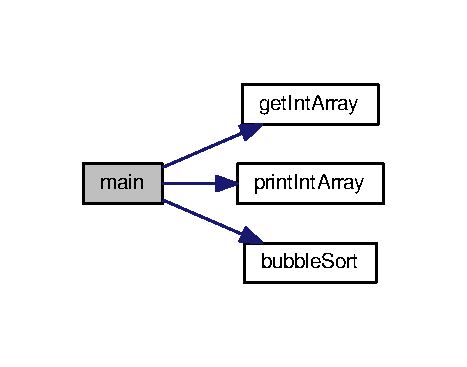
\includegraphics[width=224pt]{Bubble_8c_a840291bc02cba5474a4cb46a9b9566fe_cgraph}
\end{center}
\end{figure}


\index{Bubble.\+c@{Bubble.\+c}!print\+Int\+Array@{print\+Int\+Array}}
\index{print\+Int\+Array@{print\+Int\+Array}!Bubble.\+c@{Bubble.\+c}}
\subsubsection[{\texorpdfstring{print\+Int\+Array(int a[], int n)}{printIntArray(int a[], int n)}}]{\setlength{\rightskip}{0pt plus 5cm}void print\+Int\+Array (
\begin{DoxyParamCaption}
\item[{int}]{a\mbox{[}$\,$\mbox{]}, }
\item[{int}]{n}
\end{DoxyParamCaption}
)}\hypertarget{Bubble_8c_a84fa1f32b691605131bea795bba242bd}{}\label{Bubble_8c_a84fa1f32b691605131bea795bba242bd}

\begin{DoxyCode}
34 \{
35   \textcolor{keywordtype}{int} i;
36 
37   \textcolor{keywordflow}{for} (i=0; i<n; )\{
38     printf(\textcolor{stringliteral}{"\(\backslash\)t%d "}, a[i++]);
39     \textcolor{keywordflow}{if} (i%5==0)
40       printf(\textcolor{stringliteral}{"\(\backslash\)n"});
41   \}
42   printf(\textcolor{stringliteral}{"\(\backslash\)n"});
43 \}
\end{DoxyCode}

%--- End generated contents ---

% Index
\backmatter
\newpage
\phantomsection
\clearemptydoublepage
\addcontentsline{toc}{chapter}{Index}
\printindex

\end{document}
